\section{Trial runs}\label{trial_and_error}
Poor chain convergence was identified during trial runs, as shown in \hyperref[trace]{\textcolor{blue}{Section }\ref{trace}}. This is has been attributed to the absence of parameter transformation, as convergence improved drastically after implementing it during testing. The Methodology of these trial runs is explained in \hyperref[trial_method]{\textcolor{blue}{Section }\ref{trial_method}}. The trial runs were similar to the final runs (same models and samplers), but there were also some notable differences. 
Furthermore, MODFLOW raised an \textit{AssertionError} for some parameter sets during these trial runs. How these errors have been resolved is explained in \hyperref[sim_error]{\textcolor{blue}{Section }\ref{sim_error}}.

\subsection{Methodology}\label{trial_method}
Three samplers (DE, DE-SNK and AI) were used to calibrate four models (\hyperref[fig_logbook_1.0_CONGROMO]{\textcolor{blue}{Figure }\ref{fig_logbook_1.0_CONGROMO}}). Each model was calibrated with 3 ensembles (per sampler) consisting of 10 chains of 1500 steps each. All chains were run for 500 steps burn-in and an additional 1000 steps of main-sampling. The different samplers were initialised at the same position for fair comparison, with starting positions selected stochastically from Unif(0.0001,20). Priors for all parameters were set to N(10,10) and measurement uncertainty, which determines the likelihood function, was set to N(0,0.2). No parameter transformation was applied, so both for sampling and likelihood evaluation the same parameter values for the hydraulic conductivity (m/d) were used. 

\begin{figure}[ht]
\centering
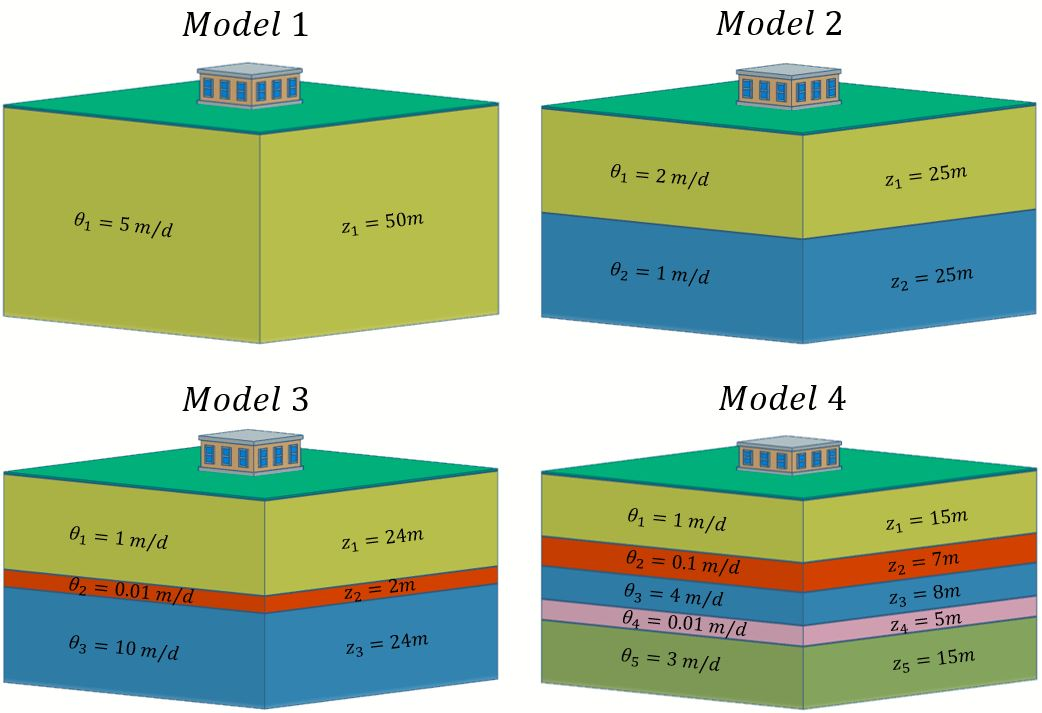
\includegraphics[width=1.0\linewidth]{Figures/CONGROMO_NEW4.JPG}
\caption{Schematic of the four steady-state synthetic groundwater flow models used in this study. Layer thickness and the respective isotropic hydraulic conductivities are shown inside each layer. The models have a length and width of 1000 meters, consisting of 25 rows and columns, with a length of 40 meters respectively. The total depth of each model equals 50 meters. At the centre of each model is an abstraction well (indicated by the building), extending over the full depth of the phreatic aquifer, with an extraction rate of 500 m\textsuperscript{3}/day. At the edges of each model, there are constant head boundaries of 10 meters.}\label{fig_logbook_1.0_CONGROMO} %so the location of the label influences how it is referenced!?, that's clunky
\end{figure} 

\subsection{Trace plots}\label{trace}
Trace plots are presented for model four to investigate whether the different moves explore the parameter space as intended. Model four was selected, because it has the highest number of parameters to be calibrated (5). The ensemble and subsequent chain selection was arbitrary. 

The first 600 steps of the AI sampler of a specific chain show little variation in parameter values (\hyperref[fig_logbook_1.1_trace_plot_Stretch]{\textcolor{blue}{Figure }\ref{fig_logbook_1.1_trace_plot_Stretch}}), suggesting high autocorrelation and low acceptance fraction for proposals. This problem appears to be even worse for the DE sampler (\hyperref[fig_logbook_1.1_trace_plot_DE]{\textcolor{blue}{Figure }\ref{fig_logbook_1.1_trace_plot_DE}}) and for DE-SNK (\hyperref[fig_logbook_1.1_trace_plot_DEsnooker]{\textcolor{blue}{Figure }\ref{fig_logbook_1.1_trace_plot_DEsnooker}}), with the chains moving only roughly every hundred steps. Another problem is that parameter 2 in \hyperref[fig_logbook_1.1_trace_plot_Stretch]{\textcolor{blue}{Figure }\ref{fig_logbook_1.1_trace_plot_Stretch}} appears to never move. 

The acceptance fraction for these specific chains has been calculated to verify whether the chains indeed exhibit the infrequent movement suggested by the trace plots, or if the moves are so small that they are not detectable in the trace plots. The acceptance fraction for different parameter within specific chains does not vary (\hyperref[tab_logbook_1.1_acceptance_frac]{\textcolor{blue}{Table }\ref{tab_logbook_1.1_acceptance_frac}}), meaning that parameter 2 in \hyperref[fig_logbook_1.1_trace_plot_Stretch]{\textcolor{blue}{Figure }\ref{fig_logbook_1.1_trace_plot_Stretch}} does move as intended, but due to the scale it is not visible. All acceptance fractions are low, as was expected based on the trace plots, with DE scoring the worst with roughly 1 in 100 proposals being accepted. These acceptance fractions are very low compared to the ideal acceptance fractions, which, as a rule of thumb, should be between 0.2 and 0.5 \citep{foreman2013emcee}. 

\begin{table}[ht]
\centering
\caption{Compares the acceptance fraction of proposed steps by different samplers (AI, DE, DE-SNK)  for calibrating Model four. The presented acceptance fractions for each parameter ($\theta$) are from the 2\textsuperscript{nd} chain of the 3\textsuperscript{rd} ensemble of each sampler.}
\label{tab_logbook_1.1_acceptance_frac}
\begin{tabularx}{\linewidth}{XXXXXX}
\toprule
 & \(\theta_1\) & \(\theta_2\) & \(\theta_3\) & \(\theta_4\) & \(\theta_5\) \\
\midrule
AI & 0.059 & 0.059 & 0.059 & 0.059 & 0.059 \\
DE & 0.011 & 0.011 & 0.011 & 0.011 & 0.011 \\
DE-SNK & 0.020 & 0.020 & 0.020 & 0.020 & 0.020 \\
\bottomrule
\end{tabularx}
\centering
\end{table}

\begin{figure}[hbt]
\centering
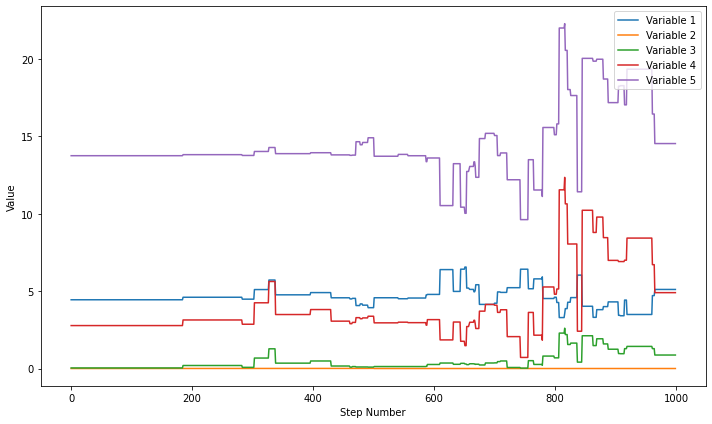
\includegraphics[width=0.9\linewidth]{Figures/appendix_figs/C.1.1 trace plot Stretch.png}
\caption{A trace plot of the Stretch move for calibrating model four. The presented chain is the 2\textsuperscript{nd} chain of the 3\textsuperscript{rd}  ensemble. Only the 1000 steps of the main sampling are presented, the 500 burn-in steps were discarded. }\label{fig_logbook_1.1_trace_plot_Stretch}
\end{figure}

\begin{figure}[ht]
\centering
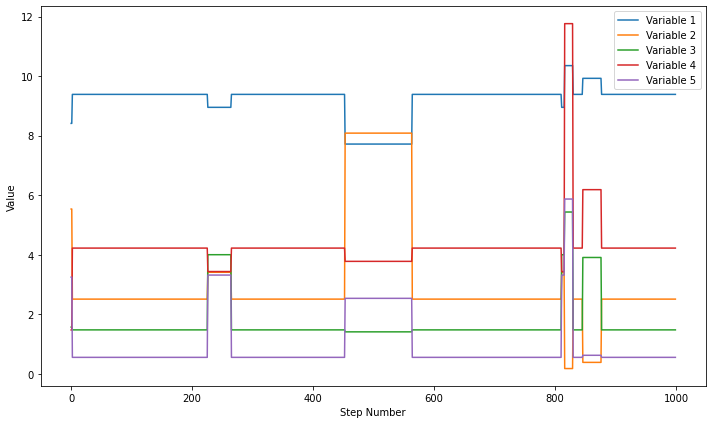
\includegraphics[width=0.9\linewidth]{Figures/appendix_figs/C.1.1 trace plot DE.png}
\caption{A trace plot of the Differential Evolution move for calibrating model four. The presented chain is the 2\textsuperscript{nd}
chain of the 3\textsuperscript{rd} ensemble. Only the 1000 steps of the main sampling are presented, the 500 burn-in steps were discarded.}\label{fig_logbook_1.1_trace_plot_DE}
\end{figure}

\begin{figure}[hb]
\centering
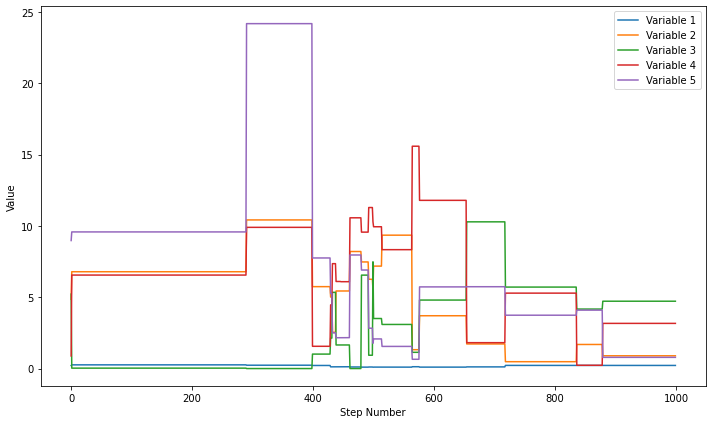
\includegraphics[width=0.9\linewidth]{Figures/appendix_figs/C.1.1 trace plot DEsnooker.png}
\caption{A trace plot of a combination
of Differential Evolution (frequency 0.8) \& snooker update (frequency 0.2) moves for calibrating model four. The presented chain is the 2\textsuperscript{nd}
chain of the 3\textsuperscript{rd} ensemble. Only the 1000 steps of the main sampling are presented, the 500 burn-in steps were discarded.}\label{fig_logbook_1.1_trace_plot_DEsnooker}
\end{figure}



\FloatBarrier
\subsection{MODFLOW simulation errors}\label{sim_error}
MODFLOW raised an \textit{AssertionError} for some parameter sets, during trial runs. In total 185 AssertionErrors were encountered in approximately 135,000 simulations (3 samplers * 3 ensembles * 10 chains * 1500 steps). AssertionErrors were encounterd from all models, with the majority from Model 4.  

%Three different samplers were compared: Goodman and Weare's affine invariant sampler with the Stretch move (AI), Differential evolution (DE) and lastly a combination of Differential Evolution (frequency 0.8) \& snooker update (frequency 0.2). All three samplers were run for three ensembles per model, with each ensemble consisting of 10 chains. All chains were run for 500 steps burn-in and an additional 1000 steps of main-sampling. The different samplers were initialised at the same position for fair comparison, with starting positions selected stochastically from Unif(0.0001,20). Priors for all parameters were set to N(10,10) and measurement uncertainty, which determines the likelihood function, was set to N(0,0.1).



These errors can be resolved in different ways. By default the selected solver is the Simple solver, where Simple indicates that default solver input values will be defined that work well for nearly linear models. This option is generally suitable for models that do not include nonlinear stress packages and models that are either confined or consist of a single unconfined layer that is thick enough to contain the water table within a single layer \citep{waterloo2024solver}. Changing the solver complexity to Moderate or Complex will resolve most errors. However, the Simple solver is most appropriate for the models designed for this thesis, as they have little complexity. 

Another possible solution is to make convergence criteria of the selected solver less strict (note that every solver has a linear and non-linear version, from which one is selected automatically). This can be accomplished by changing the values of Inner\_dvclose and Outer\_dvclose. Where, Outer\_dvclose defines the dependent-variable (for example, head or concentration) change criterion for convergence of the outer (nonlinear) iterations, in units of the dependent-variable (for example, length for head or mass per length cubed for concentrations). When the maximum absolute value of the dependent-variable change at all nodes during an iteration is less than or equal to OUTER\_DVCLOSE, iteration stops \citep{waterloo2024solver}. Inner\_dvclose is similar to Outer\_dvclose, but used by the linear solver instead. While increasing Inner\_dvclose and Outer\_dvclose does eventually resolve all errors, it requires increasing their values by three orders of magnitude (\hyperref[tab_dvclose_errors]{\textcolor{blue}{Table }\ref{tab_dvclose_errors}}). This may result in premature convergence to very different hydraulic head values in specific cells, compared to a model run with stricter convergence criteria, and was therefore deemed a poor solution. 

\begin{table}[ht]
\centering
\caption{Number of errors remaining after adjusting Outer\_dvclose and Inner\_dvclose, in MODFLOW simulations. Where, the errors refer to the MODFLOW simulation errors encountered when generating the results. And Outer\_dvclose and Inner\_dvclose are parameters set in MODFLOW6's iterative model solution (IMS) package, which is used to solve flow and/or transport simulations. Outer refers to the non-linear solver and Inner to the linear solver.}
\label{tab_dvclose_errors}
\begin{tabularx}{\linewidth}{XXX}
\toprule
Outer\_dvclose (m) & Inner\_dvclose (m) & Number of Errors Remaining \\
\midrule
0.001 (default) & 0.001 (default) & 185 \\
0.01  & 0.01 & 75  \\
0.1   & 0.1  & 18  \\
1.0   & 1.0  & 0   \\
\bottomrule
\end{tabularx}
\centering
\end{table}

Finally, the maximum allowed number of iterations was increased, allowing the numerical solver more computation time until convergence. Increasing the maximum iterations for the non-linear solver from 25 to 100 and for the linear solver from 50 to 100, decreased the number of errors from 185 to 1 (\hyperref[tab_dvclose_errors]{\textcolor{blue}{Table }\ref{tab_dvclose_errors}}). Further increasing both parameters to allow 1000 iterations each, removes the remaining error. Increasing the maximum allowed number of iterations to 1000 for IMS has little to no noticeable influence on total run time, considering that there were only 185 errors in 135 thousand model calls. Therefore, this is the solution that was implemented to generate the main results.

\begin{table}[ht]
\centering
\caption{Number of errors remaining after adjusting the parameters: Outer\_maximum and Inner\_maximum, in MODFLOW simulations. Where the errors refer to the MODFLOW simulation errors encountered when generating the results. And Outer\_maximum and Inner\_maximum are parameters set in MODFLOW6's iterative model solution (IMS) package, which is used to solve flow and/or transport simulations. Outer refers to the non-linear solver and Inner to the linear solver.}
\label{tab_maximum_errors}
\begin{tabularx}{\linewidth}{XXX}
\toprule
Outer\_maximum (iterations) & Inner\_maximum (iterations) & Number of Errors Remaining \\
\midrule
25 (default) & 50 (default) & 185 \\
100  & 100 & 1  \\
1000   & 1000  & 0  \\
\bottomrule
\end{tabularx}
\centering
\end{table}
